\documentclass[12pt]{article}

\usepackage{amsmath}
\usepackage{subfig}
\usepackage{natbib}
\usepackage{fullpage}
\usepackage{graphicx}
\graphicspath{{plots/}}
\usepackage{caption}
\usepackage{placeins}
\usepackage{xspace}
\usepackage{multirow}
  
%% MY SHORTCUTS %%
\def\numu{$\nu_{\mu}$\xspace}
\def\nue{$\nu_{e}$\xspace}
\def\thapp{$\theta_{13}$\xspace}
\def\thdis{$\theta_{23}$\xspace}
\def\dcp{$\delta_{CP}$\xspace}
\def\dm{$\Delta m^{2}_{23}$\xspace}
\def\ldsk{$\mathbf{d_{SK}}$\xspace}
\def\dsk{\mathbf{d_{SK}}\xspace}
\def\wall{\emph{wall}\xspace}
\def\towall{\emph{towall}\xspace}

\begin{document}

\section{Vertex and Direction Reconstruction Uncertainties}
\label{sec:vtxunc}

This section discribes a set of studies to estimate the detector systematics
associated with the efficiency of the FV cuts.  The error on the FV cut
efficiency depends on the data/MC agreement of the resolution of the vertex and
direction resolutions near the ID wall.  These uncertainties are not directly
addressed in the fit to atmospheric data described in TN-318.  To estimate
these uncertainties, we use the stopping cosmic muon data and the associated MC
simulation.  

An estimate of the vertex uncertainty near the ID wall is obtained by studying the
\wall distributions of the entering cosmic muon events.  Since we know the
events are entering, we know that the true \wall value as at $0$ cm.  The
vertex residual distribution projected on to the \wall direction is therefore just the
histogram of the reconstructed \wall values.  The normalized histograms for
reconstructed \wall are in Figure~\ref{fig:enteringwall}.  We
take the $68\%$ value of the cumulative distribution function
to be the measure of the vertex resolution.  Comparing this between data
and MC, we see a $2.5$ cm difference in the distribution widths.  

From this $2.5$ cm data/MC discrepancy, we estimate the effect on each T2K
sample by assuming the worst-case scenario: that each event has its vertex shifted
$2.5$ cm in the \wall direction in the same way.  We run two toy experiments: one with
the reconstructed \wall values for each event shifted by $+2.5$ cm and one 
with the reconstructed \wall values for each event shifted by $-2.5$
cm.  Comparing the difference between the two experiments, we estimate a
maximum $0.43\%$ uncertainty in the number of events in each sample. 

A similar study of the cosmic muons can be performed to estimate the
uncertainty that is introduced by adding the direction-dependant \towall
variable to define the FV cuts.  To find the systematic uncertainty for the
direction resolution, we use cosmic ray muons and their associated decay
electron. We use the direction vector that points from the muon vertex to the
electron vertex as an independent measure of the muon direction, and we compare
this vector to the reconstructed direction vector for the muon.  The data/MC
distributions are shown in Figure~\ref{fig:dirres}.  By comparing the widths of
these distributions for data and MC, we quote a systematic uncertainty for the
direction resolution of $0.24$ degrees.  Once again, we apply this uncertainty
assuming the worst-case scenario in which the direction uncertainty always
causes the \towall value to shift in the same direction for each event.  If we
shift the reconstructed direction by $0.24$ degrees in a way that increases
\towall for each event, and compare this to case where we shift the
reconstructed direction by $0.24$ degrees in a way that decreases \towall for
each event, we find the expected shift to be less than $0.067\%$.  Since this
is much smaller than the vertex uncertainty, we consider this systematic to be
negligible.  The reason the direction error is so much smaller than the vertex
error is that the data/MC agreement for the reconstructed direction is quite
good, and the density of T2K events near the \towall cut is much less than the
density of events near the \wall cut, so small shifts in the reconstructed
\towall values do not greatly effect the overall size and composition of the T2K
samples.

\begin{figure}[h!t]
  \begin{center}
    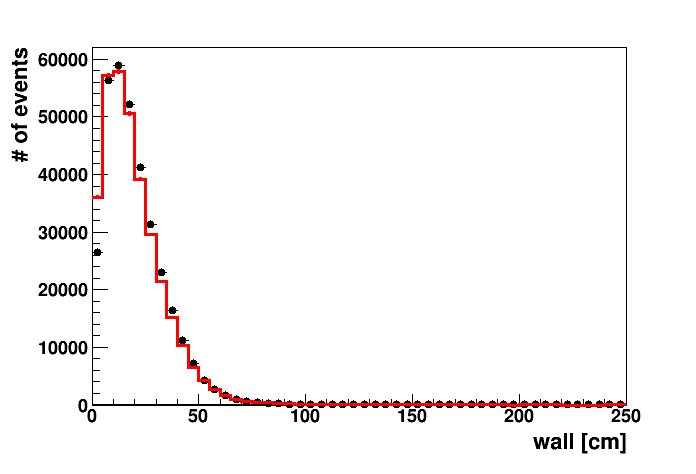
\includegraphics[width=0.4\textwidth]{cosmic_walldist}
    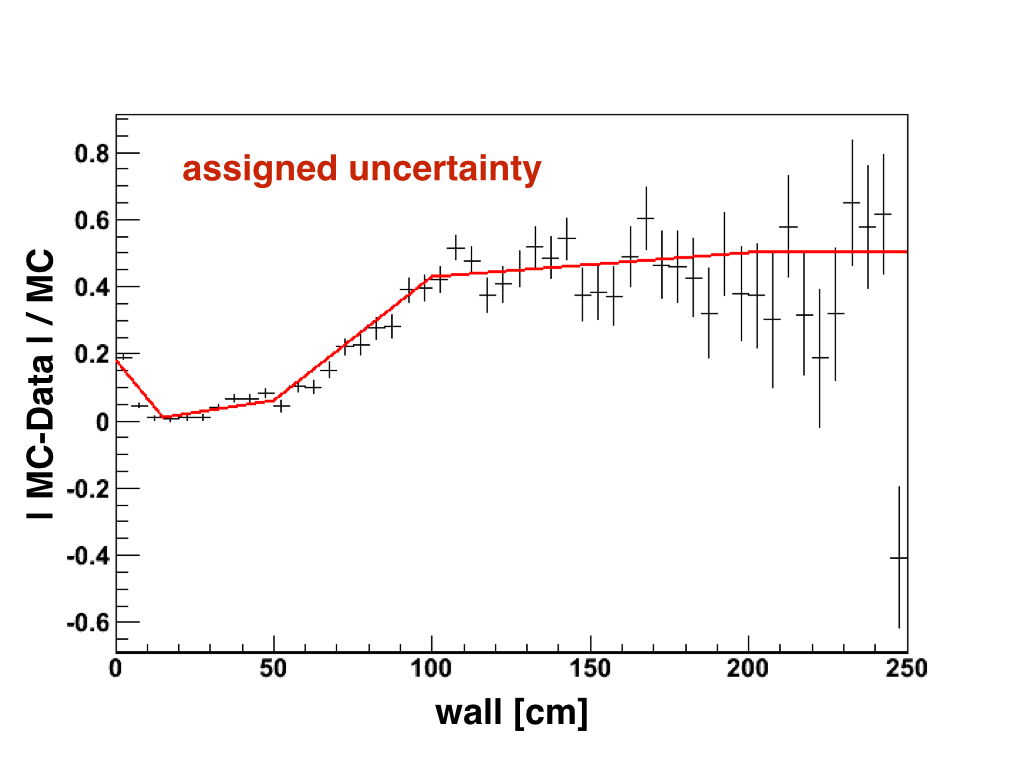
\includegraphics[width=0.4\textwidth]{entering_wall_unc}
  \end{center}
  \caption{Left plot shows the normalized \wall distributions for stopping cosmic muons.  Red histogram
  shows the MC simulation and black points show the data in each bin.  The right plot shows the absolute 
  data/MC fractional difference.  The right plot is used to apply a \wall-dependant systematic uncertainty
  for entering events.}
  \label{fig:enteringwall}
\end{figure}


\begin{figure}[h]
  \begin{center}
    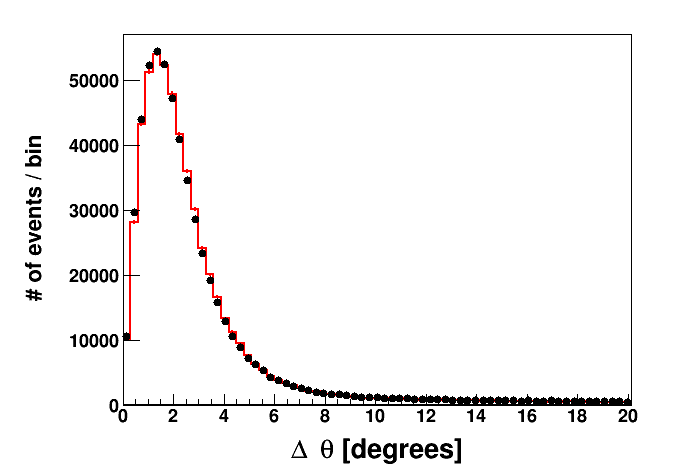
\includegraphics[width=0.5\textwidth]{cosmic_dtheta}
    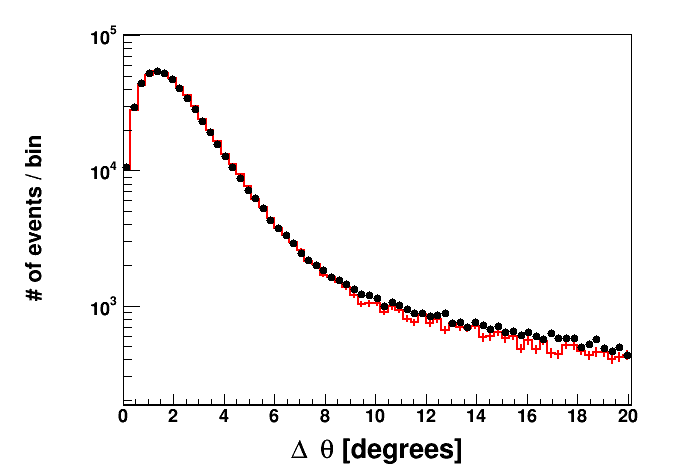
\includegraphics[width=0.5\textwidth]{cosmic_dtheta_log}
  \end{center}
  \caption{Data/MC comparison of the $\Delta \theta$: the angle between the
  reconstructed muon direction and the vector connecting the muon vertex to the
  decay electron vertex.  The data MC agreement is quite good, with only a 0.24
  degree difference in the distribution widths.}
  \label{fig:dirres}
\end{figure}

\begin{table}
  \centering
  \begin{tabular}{l | l | l}
    \hline\hline
    T2K Selection & Vertex FV Systematic [\%] & Direction FV Systematic [\%] \\
    \hline
    $\nu_{e}$ & 0.43 & 0.022\\
    $\nu_{\mu}$ & 0.31 & 0.037 \\
    $\nu_{e}$ & 0.41 & 0.067 \\
    \hline
  \end{tabular}
  \caption{Systematic uncertainties for the FV cut efficiencies estimated from
  stopping cosmic muon studies.}
  \label{tab:fverr}
\end{table}

\FloatBarrier

\section{NC $\mu$-like Charged Pion Uncertainty}

The detector systematics associated with reconstructing single charged pion rings are difficult 
to estimate.  The number of single pion events is generally small compared to the number of single muon events 
in each SK data sample, and there is no straightforward way to separate out these events without relying too 
heavily on the cuts whose efficiency we are trying to measure.  Despite these challenges, some constraints on
the uncertainty can be obtained from the Markov chain Monte Carlo (MCMC) fit to atmospheric data, which is described in 
TN-318.  Contamination from single pion events is most problematic for the T2K \numu event selection, with
14\% of the selected events coming from neutral current single pion rings (NC1$\pi$).  This section shows 
how the detector systematic uncertainty the $\mu$-like NC1$\pi$ events is calculated from the MCMC fit
to SK atmospheric neutrino data.

The strategy is to estimate the detector uncertainties using the distribution of toy Monte Carlo fake data sets.
Each fake data set is generated using a different set of detector systematics parameters, which are constrained
by the SK atmospheric data.  The detector parameterization used in this fit contains parameters that
independently shift the fiTQun likelihoods for single ring hadron events, most of which are charged pions. 
Therefore, each toy data set will have a different assumption of the single charged pion detector systematics.

The quantity we wish to estimate the uncertainty for is the efficiency of the \numu topological cuts for
selecting the NC single pion events, i.e\@:
\begin{equation}
  \varepsilon =\frac{N_{pass}^{NC1\pi}}{N_{total}^{NC1\pi}}
  \label{eq:effdefine}
\end{equation}
Calculation of the efficiency is slightly complicated by the presence
of atmospheric flux and cross section uncertainties, which are fit simultaneously with the atmospheric
data.  These flux and cross section parameters change the overall number of events in each interaction mode, so they affect
both the numerator and denominator in Equation~\ref{eq:effdefine}.  To eliminate the dependence of the efficiency
on the flux and cross section parameters, we marginalize over them:
\begin{equation}
  \varepsilon(\beta) = \int \frac{N_{pass}^{NC1\pi}(\alpha,\beta)}{N_{total}^{NC1\pi}(\alpha)}P(\alpha,\beta)d\alpha
  \label{eq:margeff}
\end{equation}
where $\alpha$ denotes the atmospheric flux and cross section parameters, and $\beta$ denotes the SK detector
systematics parameters (the shifts in the charged pion likelihood ratios, for example).  Since the MCMC fit provides 
us with samples of the $\alpha$ and $\beta$ parameters that approximate independent throws from $P(\alpha, \beta)$,
we can easily marginalize by averaging over the samples.  The quantity we calculate for the $i$-th toy MC
data set is:
\begin{equation}
  \Delta \varepsilon_{i} = \frac{1}{N} \sum\limits_{j=1}^{N}
  \frac{N_{pass}^{NC1\pi}(\alpha_{j},\beta_{i})}{N_{total}^{NC1\pi}(\alpha_{j})}
\end{equation}
The distribution of $\Delta \varepsilon$ is plotted in
Figure~\ref{fig:nc1pierr}.  From this distribution, we use the difference
between the distribution mean and the nominal value to be the ``shift error'',
and the square root of the variance of the distribution to be the ``fit
error''.  The bimodal structure in the $\Delta \varepsilon$ distribution is
caused by local maxima in the likelihood for the NC1$\pi$ $\beta$ parameters,
which arises from the limited statistics of NC1$\pi$ events.  The values of the
uncertainties are quoted in Table~\ref{tab:nc1pierr}.

\begin{figure}[h]
  \begin{center}
    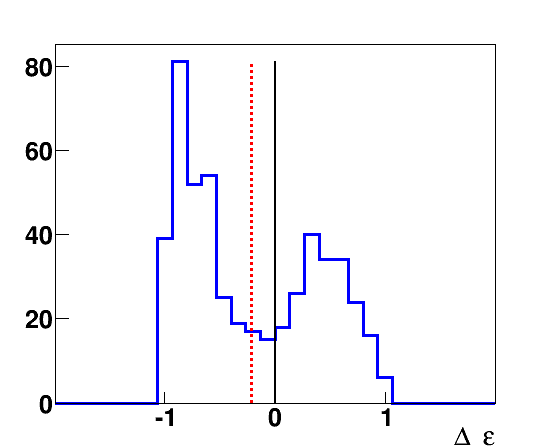
\includegraphics[width=0.5\textwidth]{ncpip_mulike_effdist}
  \end{center}
  \caption{Distribution of $\Delta \varepsilon$ over the toy MC experiments used
  to calculate the NC1$\pi$ detector uncertainty.  The red line shows the distribution
  mean, and the black line shows the nominal MC value.  The $y$-axis shows the number
  of toy experiments in each bin.}
  \label{fig:nc1pierr}
\end{figure}

\begin{table}
  \centering
  \begin{tabular}{c | c | c | c}
    \hline\hline
    Event Category & Shift Error [\%] & Fit Error [\%] & Total Error [\%] \\
    \hline
    $\mu$-like NC1$\pi$ & 61 & 22 & 65 \\
    \hline
  \end{tabular}
  \caption{Detector systematic uncertainty values calculated from Figure~\ref{fig:nc1pierr}.}
  \label{tab:nc1pierr}
\end{table}

\end{document}

